% status: 100
% chapter: Edge Computing

\title{Edge Computing and Big Data Processing using Raspberry Pi}


\author{Naveen Kaul}
\affiliation{%
  \institution{Indiana University}
  \city{Bloomington} 
  \state{IN} 
  \postcode{47408}
  \country{USA}
}
\email{nkaul@iu.edu}

% The default list of authors is too long for headers}
\renewcommand{\shortauthors}{N. Kaul}


\begin{abstract}
  Edge computing is commonly described as generation, collection, and
  analysis of data at the actual site, where data is generated as
  opposed to storing and analyzing the data at a centralized location
  like cloud or a data center. This data can be stored in a
  centralized location for a historical purposes, but the main storage
  and analysis is done on site. The technology typically consists of
  sensor-generated data, robotics, automated machines, smartphones and
  tablets, and distributed analytics servers that are used for
  computing and analysis on the spot. In this project we aim to
  explore a framework built on Raspberry Pi cluster that can be used
  to process data stored on the cluster and discuss advantages and
  limitations.
\end{abstract}

\keywords{hid-sp18-510, Edge Computing, Big Data, Spark}


\maketitle

\section{Introduction}

``Edge computing is a method of optimizing cloud computing systems by
performing data processing at the edge of the network, near the source
of the data''~\cite{hid-sp18-510-edge-wiki}. It is typically used
along with IoT (Internet of Things) devices that usually collect data,
sometimes in massive amounts. Edge computing allows devices to store
and analyze data locally, hence reducing the traffic to the central
repository/cloud.

Purpose of this project is to explore various applications of
Raspberry Pi which can be seen as next gen IoT device power source and
it becomes important to understand its limitations and
applications. This project would also implement a solution to archive
old and large files from the local cluster to a centralized cloud
location, which is a very common use case industry wide.

\section{Technologies Used}

This section describes various tools and technologies used in the
project and their configuration and implementation steps.

\begin{itemize}
	\item[$\bullet$] Raspberry Pi 
	\item[$\bullet$] Apache Spark 
	\item[$\bullet$] Google Cloud
	\item[$\bullet$] Apache Kafka	
	\item[$\bullet$] Apache Spark mllib	
\end{itemize}

\subsection{Raspberry Pi}

``A Raspberry Pi is a small credit card-sized computer originally
designed for education, inspired by the 1981 BBC
Micro''~\cite{hid-sp18-510-rpi}. It was originally created by Eben
Upton, whose goal was to create a low-cost device that can be
primarily used for improving programming skills at pre-university
level. But owing to its low cost and flexibility, it was quickly
adopted by several different people including, DIYers, makers and
electronic enthusiasts who need more than a basic microcontroller
device\cite{hid-sp18-510-rpi}.

The Raspberry Pi was designed for the Linux operating system, and
hence many Linux distributions are coming up with a version compatible
with Raspberry Pi. Raspbian and Pidora being two of the most commonly
used operating systems.

Two of the most popular options are Raspbian, which is based on the
Debian operating system, and Pidora, which is based on the Fedora
operating system. Each of these work well for beginners and can be
installed either directly on SD Cards or via NOOBS (New Out Of Box
Software) also available to download free~\cite{hid-sp18-510-rpi}.

Different models available

\begin{table}[]
	\centering \caption{Configuration}\label{t:Different Pi Models}
        \begin{tabular}{lllll} 
        \textbf{Model Name} & \textbf{Processor} 
        & \textbf{Cores} & \textbf{RAM}& \textbf{Price}
        \\ Pi Zero & 1GH 32 bit & 1 & 512 MB & \$5
        \\ Pi 1 Model A+ & 700 MHz 32 bit & 1  & 512 MB & \$20
        \\ Pi 1 Model B+ & 700 MHz 32 bit & 1 & 512 MB & \$25
        \\ Pi 2 Model B & 900 MHz 32 bit & 4 & 1 GB & \$35
        \\ Pi 2 Model B+ & 1.2 MHz 64 bit & 4 & 1 GB & \$35        
        \\
	\end{tabular}
\end{table}

\subsection{Apache Spark}

``Apache Spark is an open source big data processing framework built
around speed, ease of use, and sophisticated
analytics''~\cite{hid-sp18-510-spark}. Originally developed in 2009 in
UC Berkeley’s AMPLab, and was later open sourced in 2010 as an Apache
project~\cite{hid-sp18-510-spark}.

Characteristics of Apache Spark

\begin{itemize}
\item Spark provides a comprehensive, unified framework to manage big
  data processing requirements with support for variety of
  heterogenous data sets such as (text data, graph data etc).
\item Spark provides streaming capabilities in addition to batch
  processing.
\item Spark can improve the performance of applications up to 100
  times faster than in Hadoop by utilizing in memory processing even
  when running on disk.
\item Spark provides support for programming languages like Java,
  Scala, or Python. It also comes with a pre configured set of over 80
  high-level operators. Spark also provides a capability to
  interactively query data using spark shell.
\item It also support SQL queries, machine learning algorithms and
  graph data processing that can be used as standalone processes or
  stages in a single data processing pipeline.
\end{itemize}

\subsection{GoogleCloud}

Google Cloud Platform is a type of public cloud, which consists of a
variety of infrastructure hardware such as compute and storage
devices, and virtual resources, such as virtual machines (VMs),
Virtual Private Network etc that are contained in Google's data
centers around the globe. Each data center is located globally within
in a region. Currently, Google cloud regions include Central US,
Western Europe, and East Asia. ``Each region is a collection of zones,
which are isolated from each other within the
region''~\cite{hid-sp18-510-gcp}. Each zone is identified by a name
that combines a letter identifier with the name of the region. For
example, zone a in the East Asia region is named asia-east1-a.

Any GCP resources that a user wants to allocate or use must belong to
a project and hence project is a unique umbrella containing everything
required from hardware to lambda services. It is easier for resources
within a single project to collaborate and work together, for example
via an internal network, subject to the regions-and-zones rules.

Google Cloud platform provides a lot of services that can be broadly
classified under following categories:

\begin{itemize}
	\item Computing including hardware, containers and virtual machines
	\item Storage services
	\item Networking services
	\item Big data processing tools and technologies
	\item Machine Learning resources that also include support for
    Natural Language Processing and Computer vision related use cases.
	\item Data Analysis Services
	\item Application Platform services commonly known as PAAS (Platform
    as a Service)
\end{itemize}

\subsection{Apache Kafka}

``Apache Kafka is a publish-subscribe messaging
system''\cite{hid-sp18-510-kafka}. This means that a software through
which applications can send messages to each other. Applications can
either create messages or subscribe to the messages that are created
by other applications.  In Kafka, each message can be broadly
classified under a name called topic and kafka cluster consists of
brokers which are nodes that transfer those messages. Producers
publish data (push messages) into Kafka topics defined within the
broker and then consumer applications consume those messages from the
topic.

Messages are byte arrays that can store any object in any format. As
mentioned earlier, all Kafka messages are organized into topics and
hence any message needs to be sent or received by connecting to a
specific topic.

\begin{figure}[htbp] 
	\centering
	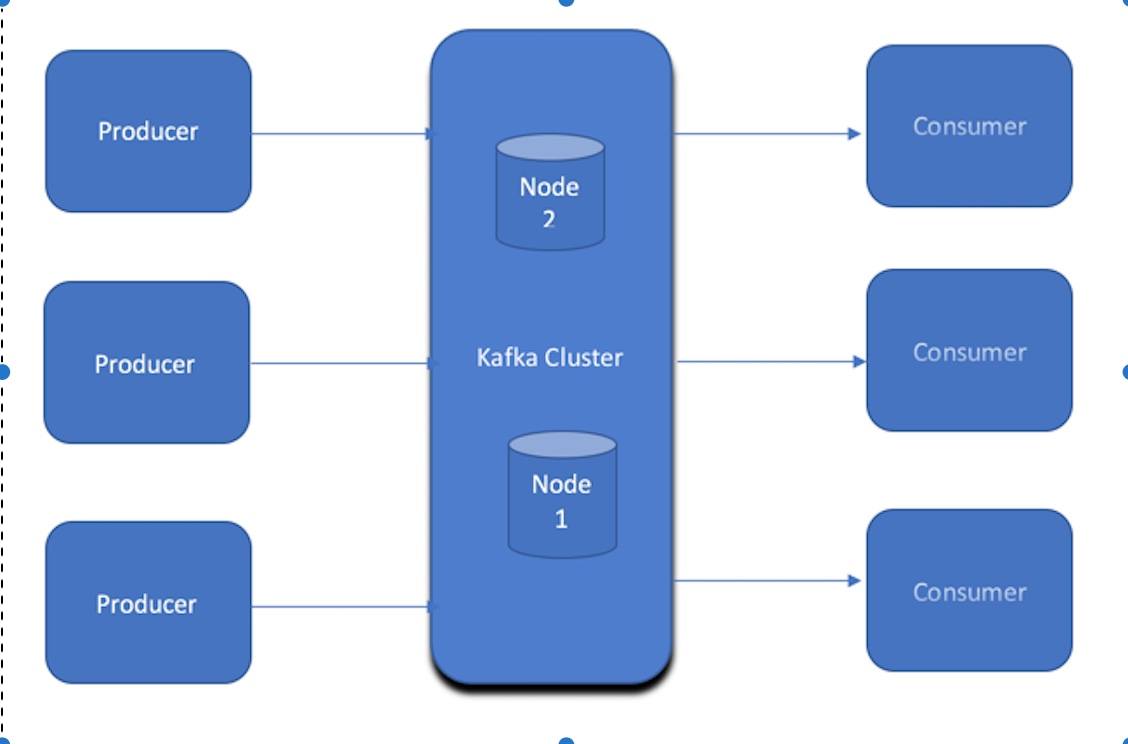
\includegraphics[width=\columnwidth]{images/kafkaarchitecture.jpg}
	\caption{Kafka Architecture}
\label{fig:kafkaarchitecture} 
\end{figure}

\subsection{Apache Spark MLlib}

The machine learning library offered by Apache Spark is called MLlib,
this is a very powerful tool to perform machine learning at scale
since this library provides support for distributed processing and
also provides a lot of machine learning algorithms out of
box~\cite{hid-sp18-510-sparkml}. MLlib very neatly into Spark's APIs
and interoperates very well with NumPy in Python and R libraries, it
can be easily used for any type of data source and efficiently plugged
into Hadoop workflows~\cite{hid-sp18-510-apmllib}.

As of latest release machine learning algorithms included in MLlib are 
\begin{itemize}
\item Classification: logistic regression, naive Bayes
\item Regression: generalized linear regression, survival regression
\item Decision trees, random forests, and gradient-boosted trees
\item Recommendation: alternating least squares (ALS)
\item Clustering: K-means, Gaussian mixtures (GMMs)
\item Topic modeling: latent Dirichlet allocation (LDA)
Frequent itemsets, association rules, and sequential pattern mining
\end{itemize}

MLlib also provides support for building data pipelines and saving
those pipelines and models for further use, providing better
reusability. It also has started providing support for third party
algorithms and packages like scikit-learn, xgboost
etc~\cite{hid-sp18-510-mllib2}.

\section{Implementation steps}

Below listed are the steps to be implemented as part of this project.

\begin{itemize}
	\item Build a hadoop/spark cluster on a cluster of Raspberry Pis.
	\item Install Zookeeper and Apache Kafka on the server
	\item Use spark cluster to train and test a machine learning algorithm
	\item Use python program to push the files to central cloud like
    Google Cloud or AWS.
\end{itemize} 

\section{Setup and Install Raspberry Pi Cluster}

Raspberry Pi is a small computer but has a lot of potential due to its
cost and applications in common day to day routines. More powerful
version of Pi can be used in industries for performing various
autonomous tasks like drones, image sensing etc. So it makes a good
use case to install big data processing tools on Pi and test its
application.

\subsection{List of Components Used}

The Pi cluster was built based on three raspberry Pis that have 1 GB
RAM and 1.2 GHz processor.

\begin{itemize}
	\item 3 Raspberry Pi B+ having 1 GB RAM and 1.2 GHz processor speed
	\item 32 GB Sandisk Micro SDXC Card
	\item Common Acrylic Case
	\item Anker Power Supply
\end{itemize}

\subsection{Installation steps}

The setup starts from procuring the hardware and then downloading the
image file from raspberry.org website. For purpose of this project,
raspbian operating system was used, which is build on debian linux
platform and comes installed with some preliminary software.

\subsection{Bootstrapping and Initial Setup}

Once the image was downloaded from raspberrypi.org, there was some
bootstrapping done so that it's easier to log into the Pis in absence
of a monitor, also sometime called as headless installation.  Below
changes were done after the image was installed Create an SSH file
Edit wpa\_supplicant.conf file to add WIFI SSID and password so that
Pi can connect to Wifi as soon as it powers on. All these steps need
to be done after the Pi has been formatted and image has been flashed
on to Pi, which can be done easily using Etcher or command line tools.

\begin{verbatim}
touch /Volumes/boot/ssh
# This will enable the ssh on Pi

nano vi /Volumes/boot/wpa_supplicant.conf
ctrl_interface=DIR=/var/run/wpa_supplicant \
GROUP=netdev
update_config=1

network={
        ssid="<network name>"
        psk="<password>"
}
# This will allow Pi to automatically 
log on to the wireless network.

\end{verbatim}

Once the Pi is powered on, as soon as it logs on to wireless network,
its IP address can be noted and then used for logging in to
Pi. Alternatively, Each Pi can also be updated with static IP
addresses or host names. Its a good idea to provide each Pi different
hostname so that they can be identified easily.

\begin{verbatim}
#Run this command after logging into each Pi
sudo vi /etc/hosts
192.168.0.1 pimaster #master node in the cluster
192.168.0.2 pislave01 #slave node1 
192.168.0.3 pislave02 #master node2 

#Edit the hostname as well for each Pi
sudo vi /etc/hostname
192.168.0.1	pimaster
\end{verbatim}

\subsection{System setup and configuration for Spark and Hadoop}

One very important setup if Spark needs to be installed on Pi, if not
done spark will not run and fail with memory issues. This also needed
to be done on all devices since spark cluster was failing repeatedly
due to memory issues.

\begin{verbatim}
sudo vi /etc/dphys-swapfile
CONF_SWAPSIZE=1000
#Pis require a reboot for the change to take effect.
\end{verbatim}

Another important step in setting up the cluster is to correctly
create and copy public keys across the cluster. It is advisable to
create another user for performing all hadoop and spark related tasks
and processes.

\begin{verbatim}
sudo addgroup hadoop
sudo adduser --ingroup hadoop hduser
sudo adduser hduser sudo
su hduse
\end{verbatim}

Run the updates on each Pi and also install required softwares

\begin{verbatim}
sudo apt-get update
sudo apt-get upgrade
sudo apt-get install python-dev python3-dev \
python-numpy python-scipy python-pandas python-matplotlib
\end{verbatim}

Next step was to create and copy keys across the cluster, for this
ssh-key-gen was run, this needs to be done for all the Pis in the
cluster so that they can communicate without any issues among each
other using SSH.

\begin{verbatim}
sudo su hduser
ssh-keygen -t RSA
ssh-copy-id hduser@pimaster
ssh-copy-id hduser@pislave01
ssh-copy-id hduser@pislave02
\end{verbatim}

Hadoop was installed directly using wget command and then copying the
folder to the desired location.  All the configurations were done as
appropriate and some of them proved to be very important.

Various websites were used as reference to performing all these
installs and some of them are listed below.

\begin{itemize}
\item tekmarathon~\cite{hid-sp18-510-pisetup-1}
\item Billion Taxi Rides~\cite{hid-sp18-510-pisetup-2}
\item Install Spark~\cite{hid-sp18-510-pisetup-3}
\end{itemize}

\section{Alternatives to using Etcher}

Since manually bootstrapping and installing all images is manageable
but this task can become cumbersome if there are a lot of nodes in a
cluster hence some mechanism of taking back up of Pi images need to be
explored.

\begin{itemize}
\item Latest raspbian operating system come preinstalled with
  SdCardcopier which is a GUI based interface to backup the image from
  a SDCard loaded on a PI to another external storage device, but even
  though this is convenient, this process still can not be performed
  via command line and needs the user to have access to Raspberry Pi
  via a monitor.
\item One way is to perform the same task as above through command
  line and even though some people have used rsync, or dd command on
  linux, they all have their disadvantages.
\item There is a command line version of SDCard copier called
  pi-clone, whose source code is available on github, but this should
  be used with caution and used only by very seasoned
  users~\cite{hid-sp18-510-git}.
\end{itemize}

\section{Installing Spark}

Spark can also be installed correctly from apache website and version
used in this project was 2.3.0. One very important thing to keep in
mind while installing Spark is that spark needs a lot of memory to
work that can not be provided by Raspberry Pi as they only have 1 GB
Ram for B+ and even less than that in all other models so there are
some configurations that needs to be modified before Spark can
function properly.~spark-env.sh located at \$SPARK\_HOME needs below
settings

\begin{verbatim}
SPARK_MASTER_HOST=pimaster
SPARK_WORKER_MEMORY=512m
SPARK_EXECUTOR_MEMORY=512M
SPARK_DRIVER_MEMORY=512M
HADOOP_CONF_DIR=$HADOOP_HOME/etc/hadoop
SPARK_DAEMON_MEMORY=512m
\end{verbatim}

After successful installation of hadoop and spark, their activity 
can be monitored through the URLs. Default url for spark is 
//master-node:8080

\begin{figure}[htbp] 
	\centering
	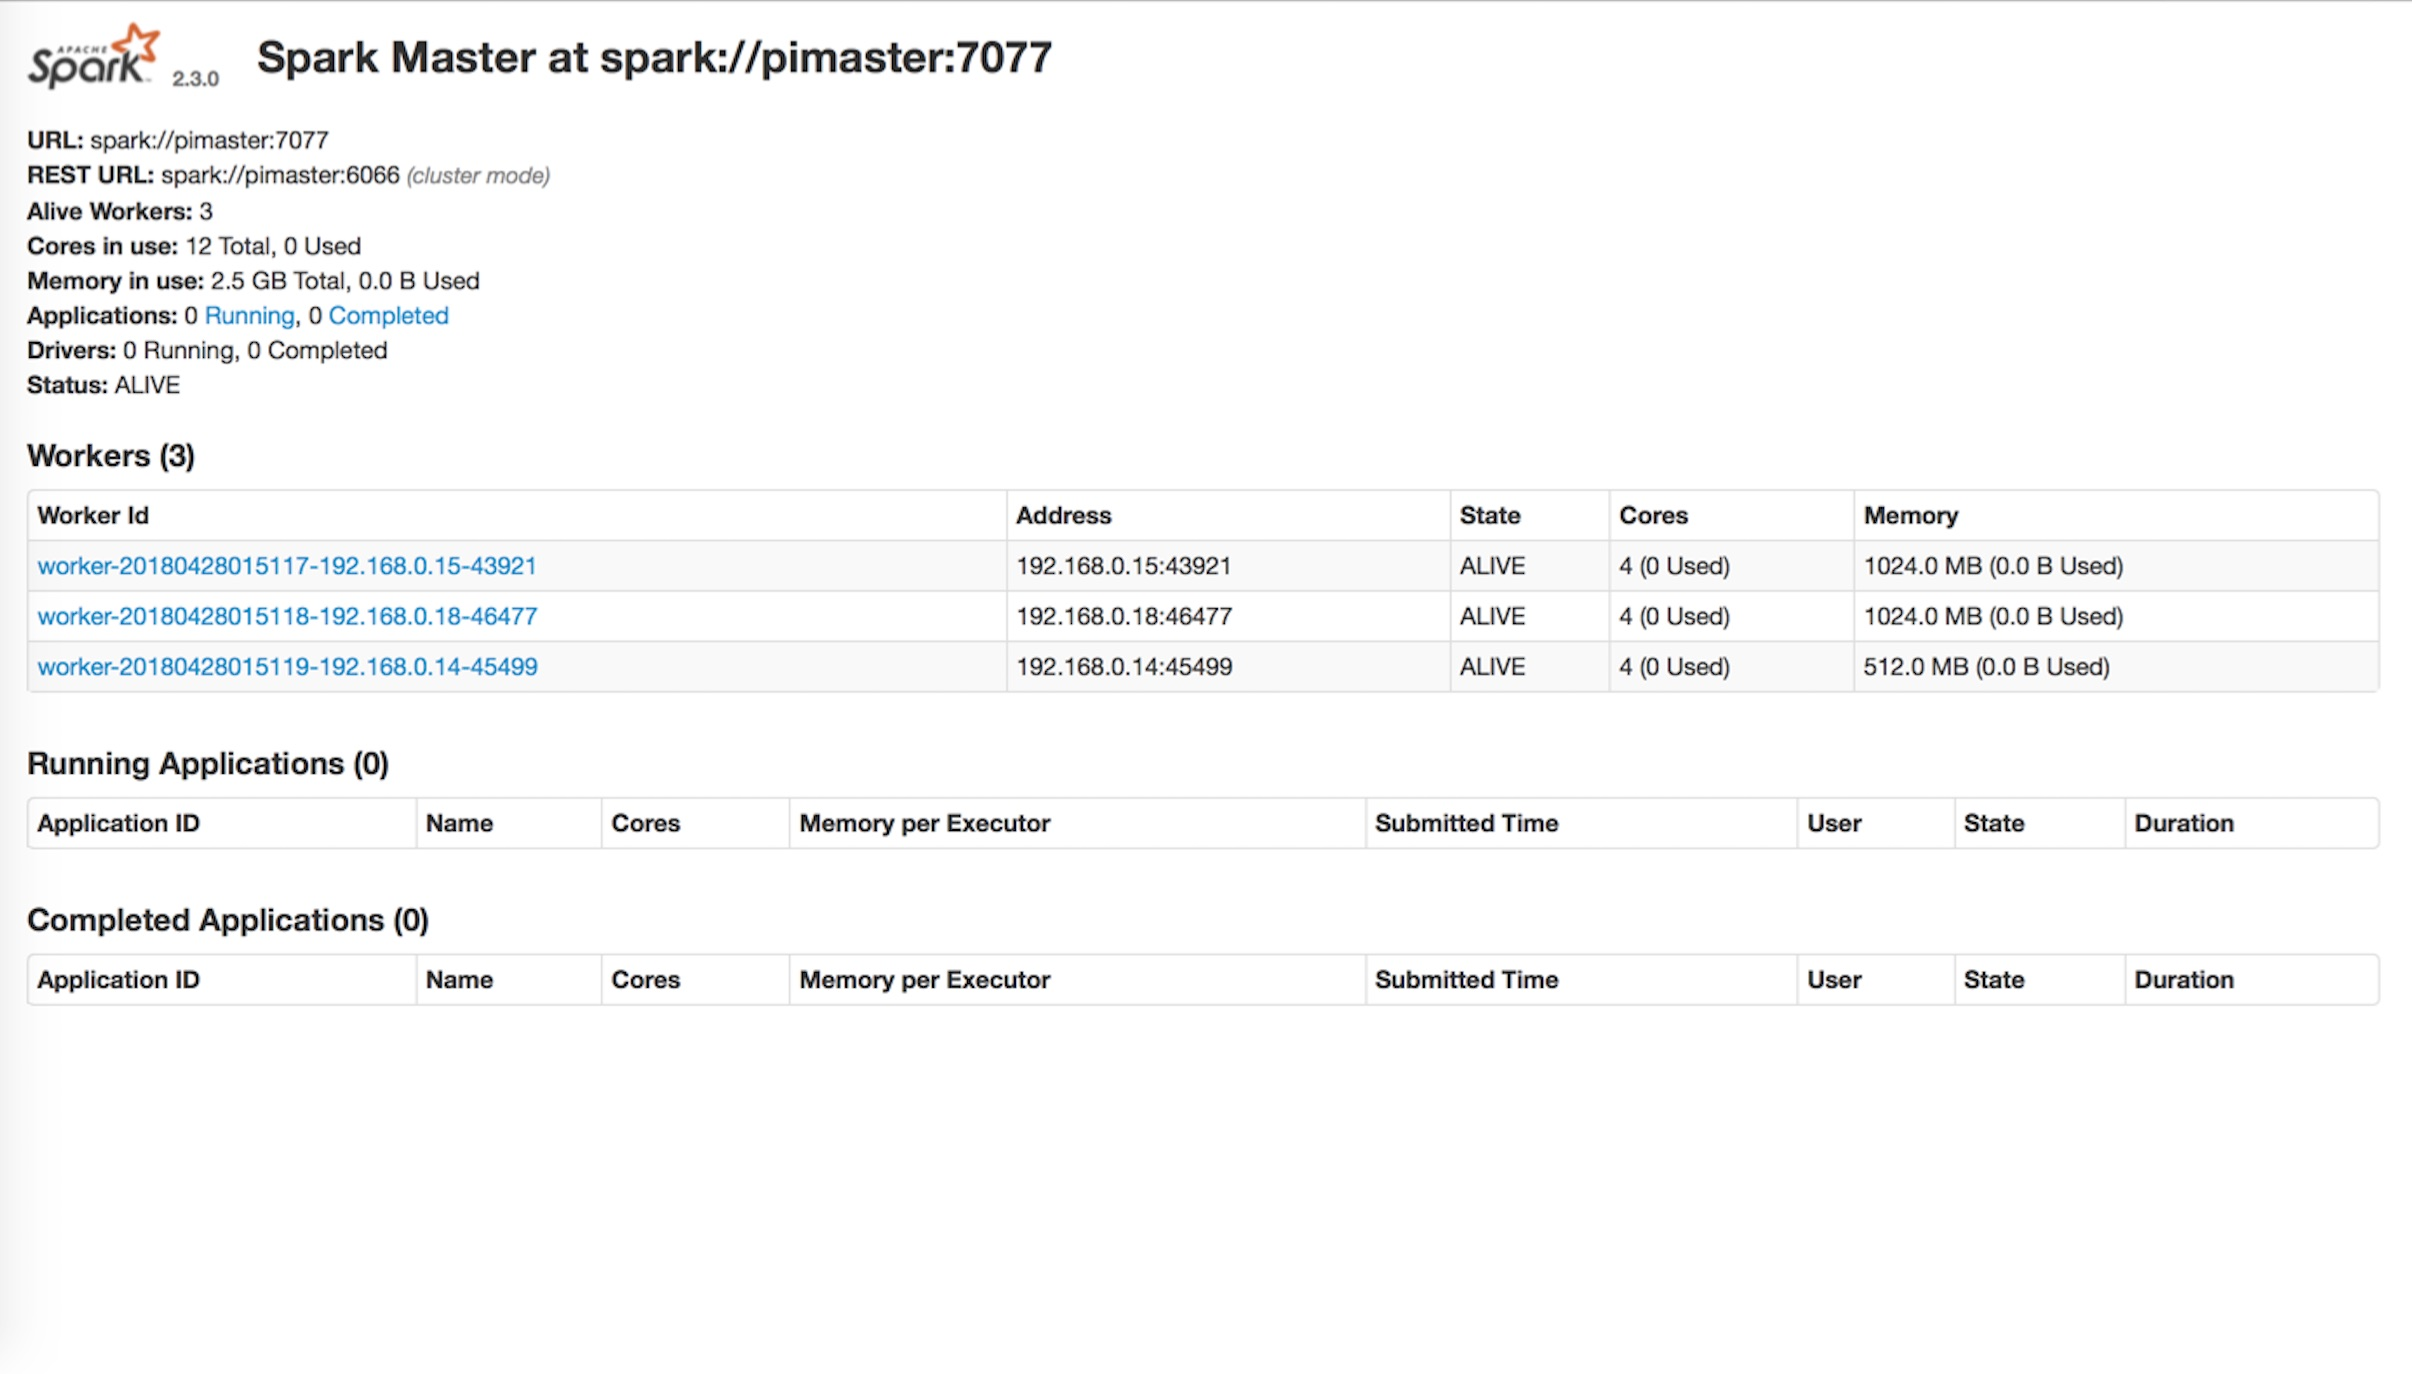
\includegraphics[width=\columnwidth]{images/sparkurl.jpg}
	\caption{Sample SPARK Url}
\label{fig:sparkurl} 
\end{figure}

\subsection{Running Spark}

There are several ways that Spark can be run either through
spark-submit or spark-shell mode. In an order for Spark to run in
cluster mode, HADOOP\_CONF\_DIR or YARN\_CONF\_DIR need to be set so
that Spark processes know how to communicate with Hadoop and Yarn.

Spark can be started by running

\begin{verbatim}
$SPARK_HOME/bin/start-master.sh
$SPARK_HOME/bin/start-slaves.sh
\end{verbatim}

Once started, verification can be done using spark-shell or pyspark
commands if the pyspark is installed.

Sample command line view

\begin{verbatim}
Spark session available as 'spark'.
Welcome to
      ____              __
     / __/__  ___ _____/ /__
    _\ \/ _ \/ _ `/ __/  '_/
   /___/ .__/\_,_/_/ /_/\_\   version 2.3.0
      /_/
         
Using Scala version 2.11.8 (Java HotSpot(TM) 
Client VM, Java 1.8.0_65)
Type in expressions to have them evaluated.
Type :help for more information.
\end{verbatim}

\section{Machine Learning on Pi cluster}\

The main topic of this project is to determine whether we can use
Raspberry Pi for performing any AI or Machine learning related task
since its small, cheap and yet powerful so some machine learning and
few deep learning algorithms were attempted on the cluster and their
performance was monitored and compared. One thing can be said without
doubt that Raspberry Pi can not be yet used for Deep Learning
capabilities with limits on memory and processing power. Some deep
learning applications were tried to classify images of flowers and Pi
master node became unresponsive while the model was run and hence had
to be killed. A normal machine learning algorithm runs within seconds
on a cluster if 3 Pis but does not scale very well even with Spark
installed. Main issue being available memory since swap space alone
can not accomodate for less memory.

The machine learning algorithm run was a linear regression algorithm
to predict the median price of houses in different districts of
California. The job took around 1 minute to train on a dataset of
20,000 records, which barely takes seconds when run on a powerful
personal computer like Mac or Windows.

\subsection{Predicting House prices }   

Dataset~\cite{hid-sp18-510-dataset} needs to be downloaded from the
website directly. This dataset can be stored locally and then loaded
in SPARK RDD by running below command

\begin{verbatim}
rdd = sc.textFile('/path/cal_housing.data')
\end{verbatim} 

Various commands can be run to analyze contents of the dataset like 
\begin{verbatim}
describe()
collect() Running collect is not advisable since that can take
  up all the driver memory and cause Spark to fail
show()
take()
\end{verbatim}

Since looking at data it seems that the data is not uniformly
distributed so it becomes very important as with any other machine
learning algorithm to standardize the data using Scaler functionality
of Spark MLlib. It standardizes features by either scaling data to
unit variance and/or scaling data based on the man and standard
deviation of the dataset.

\begin{verbatim}
standardScaler = 
StandardScaler(inputCol="features", outputCol="scaled_features") 
scaler = standardScaler.fit(df)
scaled_df = scaler.transform(df)
\end{verbatim}

Data can then be split into training and test dataset randomly 
usually in a 80\%-20\% split, model is trained on 80\% of data 
while tested on rest of 20\%. 

A few other things that can come handy for machine learning using 
edge devices are

\begin{itemize}
\item Using pre-trained model which can be fitted or trained on high
  performance machines and then deployed on these devices, these
  devices can then use those models to make predictions and also send
  any new data back to the central location
\item MLlib provides an option of online learning where machine
  learning can also be applied on the data being streamed which can
  reduce latency and burden on the processing power by taking into
  account all the data points but at different times.
\end{itemize}

Sample code snippets for machine learning were utilized from
DataCamp\cite{hid-sp18-510-dc}.

\section{Data Storage/Archival}

Since storage is very limited on the pi cluster and even the edge
devices that are commonly used, they can not afford to store a lot of
data so one good option is to archive data at regular intervals or
based on the size to a central cloud location like AWS, Azure or
Google Cloud. In this project, various options provided by Google
Cloud were explored.

Google Cloud platform provides different storage solutions based on
different applications and workloads requirements.

Some of the main products that make sense from the topic at hand are

\begin{itemize}
\item Persistent Disk - Fully managed storage used for taking backup
  of virtual machine, this can be a good option for the edge devices
  that have some container installed on them.
\item Google Cloud Storage - This is a good option for storing images
  and media files.
\item Google Cloud Big Table - This is also a good option for IoT
  devices that do not have standard data structures like rows and
  columns since this storage can also use noSQL databases etc.
\end{itemize} 

\subsection{Methods to transfer Data}

Google Cloud storage platform provides various ways to transfer data
between various cloud resources and other servers. These include JSON
or XML based APIs or even command line utilities to perform such tasks.

\subsection{JSON APIs}

Any cloud service including Google Cloud Platform provide JSON APIs
that can be called programmatically to store objects in the cloud
remotely using HTTP.

Steps required to upload objects in Google Cloud using JSON APIs
\begin{itemize}
\item Get an authorization access token from the OAuth 2.0
  Playground. Configure the playground to use your own OAuth
  credentials.
\item Add the object's data to the request body.
\item Use cURL to call the JSON API with a POST Object request
\end{itemize} 

\begin{verbatim}
curl -X POST --data-binary @file_name \
    -H "Authorization: Bearer Token_Key" \
    -H "Content-Type: Object" \
\end{verbatim}

\subsection{Command Line Utilities}

Google also provides command line utility called gsutil which can be
used to perform several options in cloud storage.

Creating a bucket which is a storage container on Cloud

\begin{verbatim}
gsutil mb -l us-east1 gs://my-bucket/
\end{verbatim}

Copying objects from local folder to cloud

\begin{verbatim}
gsutil cp my-local-folder/my_file gs://my-bucket/my-folder/
\end{verbatim}

\section{Challenges Faced}

While working on this project, there were several challenges that had
to be overcome in order to achieve the final goal. Some of them are 
listed below. 

\subsection{Change in filename from slaves to workers on hadoop 3.1.0}

There has been a change in the file name for defining the host names
of slaves and master in Hadoop from 3.1.0, workers file has to be used
compare to slaves file in previous versions, this created some
confusion and as a result workers not being started on the hadoop
cluster.

\subsection{Spark cluster failing due to memory issues}

Spark cluster kept failing with memory issues initially and created a
lot of issues in running any machine learning algorithms. This problem
was only solved after referencing a lot of forums and online
discussions to understand the configuration changes. Changing swap
file size helped too.

\subsection{Running deep learning libraries on Pi cluster}

Running deep learning algorithms like Theanos, Keras and TensorFlow on
Pi cluster was also unsuccessful primarily due to memory size and
incompatibility of some libraries with Pi operating system. A lot of
attempts were made to have these libraries work but could not be
completed successfully within the available time.

\subsection{Issue in running jupyter with spark on pi}

There were also some compatibilities with jupyter and spark on Pi
since some libraries were not compatible with each other. Also in
order to run jupyter on any of Pi, it can be done by using VNC and
remotely logging into the server or connecting a monitor to the Pi.

\section{Next Steps}

While, this project started with setting up a hadoop and spark cluster
on raspberry pi, an effort was made to also try various deep learning
libraries on spark like Keras and TensorFlow but those objectives could 
not be achieved due to memory limitations of Raspberry Pi. Below are 
some of ideas that can be used to enhance the project.

\subsection{Running DeepLearning on Pi cluster}

As discussed earlier, running deep learning libraries on Pi cluster
can be very beneficial from the use case of edge computing so making
those work successfully is a good step in moving towards broadening
the usage of Pi.

\subsection{Streaming Data from Sensors}
Apache Kafka can be easily used to stream data from several add-on sensors 
on Pi and this data can then be used to perform some actions using the Pi.
For example, if sensor detects heat, Pi can send a message or email to user
in order to alert them, similarly a camera can be easily installed on Pi
and then used for streaming images and making decisions based on the images.

\section{Conclusion}

While Raspberry Pi individually or as a cluster has a lot of potential
to be used for edge devices, it can not be treated as a one stop shop
for all kinds of problems. It can be used very well for use cases
where we need a device which is more complex and flexible than a
simple microcontroller but costs less than a server, but use cases
where there is lot of data processing involved, which requires a lot
of in memory processing, it may fall short of in achieving its full
potential. Nevertheless Raspberry Pi is a very nifty tool, but it has
a long way to be used in the industry.

\bibliographystyle{ACM-Reference-Format} 
\bibliography{report}

